\chapter{Referencial Teórico/ Revisão Bibliográfica}

\section{Inteligência Artificial e Sistemas Multiagentes}

A Inteligência Artificial (IA), na sua origem, focou na criação de sistemas autônomos com a capacidade de resolver problemas com a ajuda mínima de outros sistemas. Esses sistemas muitas vezes não eram suficientes quando a resolução do problema não se adequava a sua especialização. A solução foi colocar o sistema em uma sociedade de sistemas com uma coleção diversificada de habilidades e capacidades, da mesma forma que as pessoas superam as limitações dos indivíduos quando trabalham juntas em uma organização \cite{durfee1991distributed}. 

Assim surgiu a IAD uma subárea da IA que concentra esforços na pesquisa da compreensão das técnicas de conhecimento e raciocínio necessárias para a coordenação inteligente e sobre a incorporação e avaliação deste entendimento em sistemas de informação. Outros fatores também contribuíram e permitiram o desenvolvimento desta subárea, como o surgimento da computação distribuída e dos \textit{clusters} de computadores \cite{durfee1991distributed,bond2014readings}.

Segundo \cite{durfee1994distributed} da IAD surgiram duas novas subáreas:

\begin{itemize}
\item Resolução Distribuída de Problemas (RDP): onde o sistema tem ênfase na resolução de um problema e como fazer com que vários agentes trabalhem juntos para solucioná-lo de forma coerente, robusta e eficiente.

\item SMA: baseado na teoria dos jogos e na ciência social tem o pressuposto que o agente deve ser autônomo, racional, ter conhecimento do ambiente e de outros agentes garantindo mecanismos de comunicação e organização indiferente do problema a ser resolvido.
\end{itemize}

\subsection{Agente}

Atualmente não existe uma definição comum de agentes para toda a comunidade de IAD. Uma das definição mais aceitas foi proposta por \citet{ferber1991agent}:
\begin{quotation}
"Um agente é uma entidade real, ou virtual, imersa em um dado ambiente onde ela pode executar algumas ações, estar habilitada para perceber e representar parcialmente este ambiente, podendo ainda comunicar-se com os demais agentes do ambiente. Este agente apresenta um comportamento autônomo que é uma consequência de suas observações, do conhecimento armazenado e das interações com os demais agentes do ambiente."
\end{quotation}

Outras definições de agentes são apresentadas por \cite{wooldridge1995intelligent,franklin1996agent,russell2002artificial}, mas independente do tipo de agente e ambiente em que ele está inserido. Outro consenso na definição de agente é a propriedade de autonomia. A Figura \ref{fig:agente} representa um agente simples e sua interação com o ambiente.

\begin{figure}[ht]
\centering
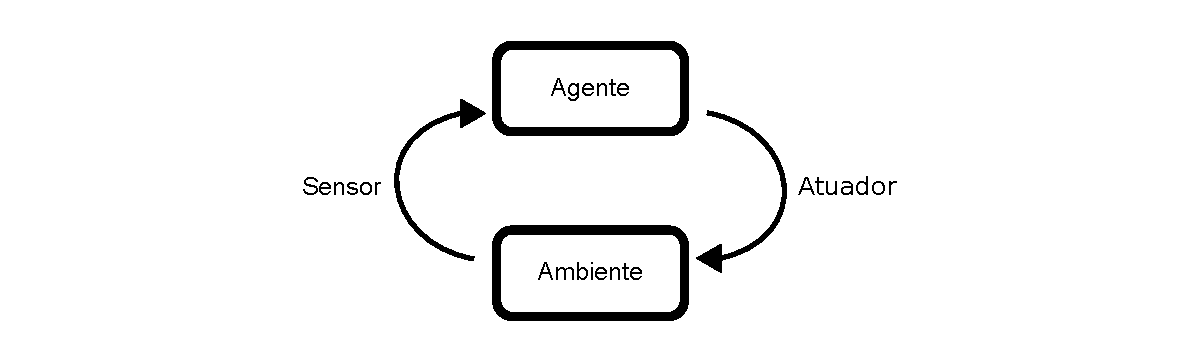
\includegraphics[scale=0.8]{imagens/agente.pdf}
\caption{Agente interagindo com o ambiente através dos sensores e atuadores, adaptado de \cite{russell2002artificial}.}
\label{fig:agente}
\end{figure}

Dois tipos de uso para “agente” são descritos por \citet{wooldridge1995intelligent}. Para o primeiro um conceito fraco de agentes e mais incontestável teriam as seguintes propriedades:

\begin{itemize}
\item Autonomia: os agentes operam sem intervenção direta de humanos ou outros agentes, e possuem algum mecanismo para controle de suas ações, o estado interno;
\item Habilidade Social: agentes interagem com outros agentes e possivelmente humanos através de uma linguagem de comunicação;
\item Reatividade: agentes percebem o ambiente e respondem rapidamente se alguma alteração ocorrer;
\item Pró-atividade: agentes podem exibir comportamento orientado a objetivo e tomar a iniciativa, não agindo apenas por reação ao que ocorre no ambiente.
\end{itemize}

Outros pesquisadores quiseram dar um significado mais forte para agente, além das propriedades já apresentadas acima, incluindo outras características como:

\begin{itemize}
\item Mobilidade: habilidade de um agente de se mover de um local para outro na rede;
\item Veracidade: um agente não envia conscientemente uma informação falsa;
\item Benevolência: os agentes não devem apresentar um comportamento contra-produtivo, e ele deve sempre executar o que foi solicitado;
\item Racionalidade: um agente atuará para alcançar seus objetivos e não agirá de forma a evitar que seus objetivos sejam alcançados, pelo menos na medida em que suas crenças o permitam.
\end{itemize}

\subsection{Classificação dos Agentes}

Assim como não existe uma definição única para agentes também não existe um único modo de classificação de agentes. Neste trabalho será apresentada a proposta de \citet{nwana1996software} que apresentou sua classificação de agente baseada nas diferentes dimensões. As dimensões expostas foram:

\begin{itemize}
\item Mobilidade: capacidade ou não de um agente se movimentar por uma rede ou ambiente;
\item Raciocínio: se o agente é deliberativo, agente que possui mecanismos para raciocinar, memorizar ações passadas, ou reativo, aquele que realiza uma ação baseado apenas no que ele percebe do ambiente;
\item Autonomia: se os agentes podem operar sem intervenção humana, ou de outro agente;
\item Aprendizagem: é a capacidade do agente em melhorar seu desempenho com a interação com o ambiente;
\item Cooperação: os agentes possuem habilidade social, e interagem com outros agentes.
\end{itemize}

 Conforme \cite{nwana1996software} a classificação dos agentes foi criada  combinando as dimensões cooperação, autonomia e aprendizagem, derivando assim sete tipos de agentes: agentes colaborativos, agentes de interface, agentes colaborativos e com aprendizagem e agentes inteligentes sendo os principais, e os tipos  agentes móveis, agentes reativos e agentes híbridos como secundários, todos representados na Figura \ref{fig:class_agente}. As distinções não são definitivas e os agentes pode ainda ser agentes heterogêneos, que é quando os agentes combinam duas ou mais categorias.



\begin{figure}[ht]
\centering
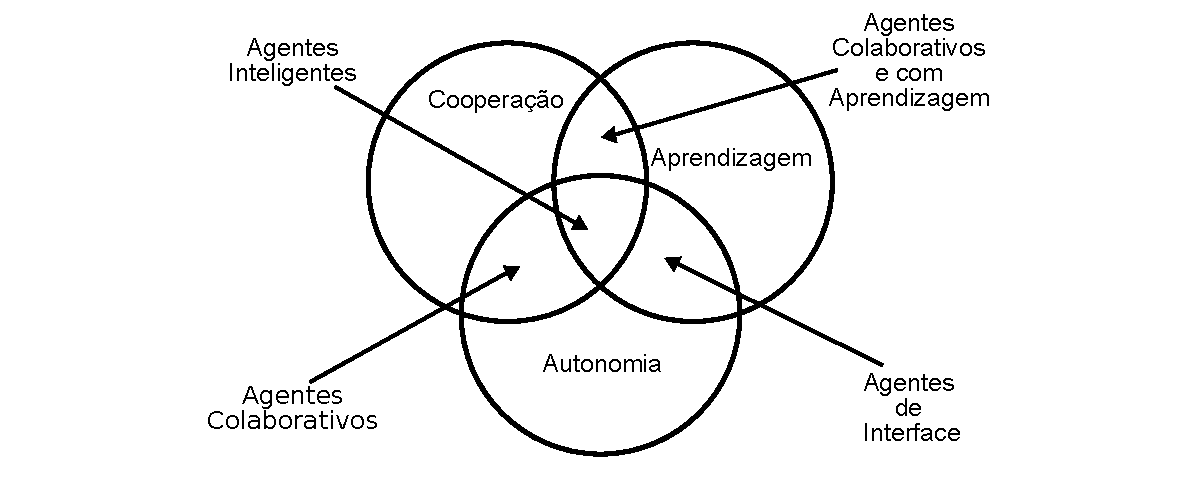
\includegraphics[scale=0.7]{imagens/tipos_agentes.pdf}
\caption{Classificação dos agentes, adaptado de \cite{nwana1996software}.}
\label{fig:class_agente}
\end{figure}

%\subsection{Arquiteturas de Agentes}




\subsection{Sistema Multiagente}

De acordo com \cite{lesser1999cooperative} sistemas multiagentes são sistemas computacionais em que dois ou mais agentes interagem ou trabalham em conjunto para executar algum conjunto de tarefas ou para satisfazer um conjunto de metas. O comportamento destes agentes pode ser limitado através de políticas nos agentes ou através de uma organização, em um acordo de que agentes específicos exercem certas funções dentro desta sociedade.

Quando os agentes interagem geralmente há algum tipo de organização que define o tipo de relação entre os agentes e influencia o seu comportamento. Estas regras de interação podem ser dinâmicas causando assim alteração no tipo de relação entre os agentes. 

Na Figura \ref{fig:sma_org} pode ser observado que os agentes estão formandos pequenos grupos chamados de organização, estas organizações podem ter características que modelam o comportamento dos agentes inclusive como eles interagem entre si, criando regras para determinar quem pode ou não se comunicar com outros agentes ou grupos. Os agentes estão inseridos em um ambiente que provê recursos, limitações ou outras características que podem beneficiar ou limitar os agentes para concluírem seus objetivos  \cite{jennings2000agent}. 

\begin{figure}[ht]
\centering
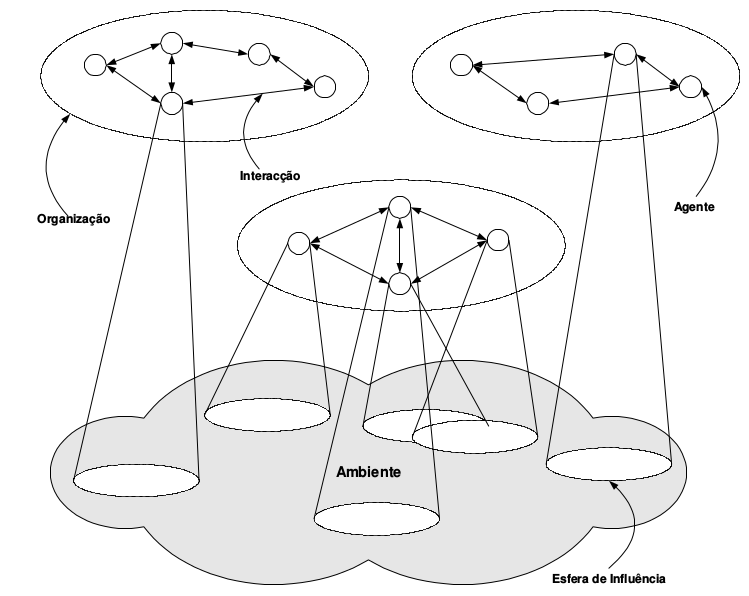
\includegraphics[scale=0.4]{imagens/sma_org.png}
\caption{Estrutura de um sistema multiagente \cite{jennings2000agent}.}
\label{fig:sma_org}
\end{figure}

\subsection{Ambiente}

O ambiente é uma abstração que dá condições para que os agentes existam, fornece recursos externos e a infraestrutura de comunicação, dando suporte para a organização e coordenação. O ambiente é uma parte essencial para o SMA, permitindo uma abstração de projeto separando as responsabilidades ajudando a gerenciar a complexidade da engenharia de software em SMA \cite{weyns2007environment}.
  
Um agente tem um certo número de ações à disposição para cumprir sua meta, mas nem sempre todas estão disponíveis. Alguma das ações podem ter condições prévias informando em que situações estas podem ser aplicadas, e estas limitações podem estar diretamente relacionadas com alguma das propriedades do ambiente. \citet{russell2002artificial} propõem uma classificação para as propriedades do ambiente.
  
\begin{itemize}
\item \textbf{Totalmente observável \textit{vs.} parcialmente observável.} \\
Se os sensores do agente dão acesso ao estado completo do meio ambiente, detectando todos os aspectos relevantes para a escolha da ação então a tarefa do ambiente é totalmente observável. Nestes tipos de ambientes o agente não precisa manter nenhum estado interno para acompanhar o mundo. Um ambiente pode ser parcialmente observável devido aos sensores do agente serem ruidosos e imprecisos, ou porque partes do estado do ambiente estão faltando nos dados do sensor, não tendo assim informações completas do estado. Quanto mais observável é um ambiente, mais simples é criar agentes para operar nele.

\item \textbf{Determinista \textit{vs.} Estocástico}\\
O ambiente é determinista se o próximo estado do ambiente for completamente determinado pelo estado atual e pela ação executada pelo agente. Não gerando assim surpresas sobre o estado que resultará a realização de uma ação por um agente. Um ambiente estocástico está associado a uma probabilidade de conhecimento do próximo estado, baseado no estado atual e na ação realizada. Se um ambiente é determinista exceto pela ação dos outros agentes então o ambiente é estratégico.

\item \textbf{Episódico \textit{vs.} Sequencial} \\
Em um ambiente episódico a escolha da ação em cada episódio depende apenas do próprio episódio, como por exemplo uma tarefa de classificação como detectar peças defeituosas em uma linha de montagem, essa ação não tem interferência de decisões anteriores, e não afetará decisões futuras. Em ambientes sequenciais a decisão atual pode afetar todas as decisões futuras, como por exemplo em um jogo de xadrez. Os ambiente episódicos são mais simples na questão de desenvolvimento.

\item \textbf{Estático \textit{vs.} dinâmico} \\
Um ambiente estático permanece inalterado, exceto por algo que ocorra em consequência da ação do agente. Neste tipo de ambiente o agente não precisa continuar observando o mundo enquanto decide uma ação e não precisa se preocupar com a passagem do tempo. Em um ambiente dinâmico pode ocorrer mudanças enquanto o agente está deliberando, ou seja, outros processos estão operando nele.

\item \textbf{Discreto \textit{vs.} Contínuo} \\
O ambiente discreto tem um número finito de estados distintos, como um jogo de xadrez, que possui um número finito de casas e jogadas possíveis. Já em um ambiente contínuo as ações ocorrem ao longo do tempo, como por exemplo uma corrida de táxi em que as ações e a localização se alteram de acordo com o tempo.

\item \textbf{Agente único \textit{vs.} Multiagente}
O ambiente onde um agente resolve um problema sozinho está em um ambiente de agente único, como é o caso de um  agente que retira as peças danificadas na linha de produção. Um agente tem por objetivo concluir sua meta de melhor maneira possível, em um ambiente multiagente podemos ter agentes atuando com comportamentos cooperativo ou competitivo de acordo com a situação desejada.
\end{itemize}

\subsection{Organização}\label{sec:orgsma}

Na nossa sociedade temos diversas organizações, e elas mostram um mecanismo eficaz para coordenar comportamentos de diferentes agentes em uma comunidade. No domínio dos sistemas multiagente a organização é uma coleção de papéis, relacionamentos e estruturas de autoridade que regem seu comportamento. Geralmente os SMA têm alguma forma de organização, embora possa ser implícita e informal. As organizações de agentes orientam o modo como os membros da população interagem uns com os outros, não apenas a curto prazo, mas também a longo prazo. Essa orientação pode influenciar as relações de autoridade, fluxo de dados, alocação de recursos, padrões de coordenação ou qualquer outra série de características do sistema \cite{horling2004survey}.

Existem vários modelos de organização e eles estruturam o comportamento de entidades complexas em uma hierarquia de entidades encapsuladas onde cada membro tem funções a desempenhar. As funções ou papéis estruturam os departamentos, e estes estruturam uma organização. A teoria da organização analisa como estas organizações funcionam, suas principais características, as características mais relevantes dos membros, os papéis gerais que os membros adotam, os relacionamentos entre os membros, a hierarquia, as regras e normas que regem a organização \cite{argente2006multi}. A organização pode ajudar grupos de agentes simples a exibir comportamentos complexos e ajudar agentes sofisticados a reduzir a complexidade de seus raciocínios.

No início, os sistemas tinham apenas uma visão centrada nos aspectos individuais dos agentes de modo que o SMA é projetado em termos de estados mentais dele, como as crenças, intenções e objetivos, conhecida como metodologia orientada a agentes. Desde então os SMA evoluíram para a metodologia orientada para a organização, levando em conta suas principais metas, estrutura e normas sociais\cite{argente2006multi}. 

Um conceito do tema de organização é a coordenação e \citet{malone1994interdisciplinary} a define como gestão de dependências entre atividades independentes. Esta definição para coordenação tem um sentido inclusivo para diferentes áreas de conhecimento, podendo ser aplicado em teoria organizacional, economia, ciência política, biologia, entre outros. Para a computação, as dependências entre diferentes processos computacionais se assemelham a interações entre pessoas, e devem ser estudados como podem ser gerenciadas.

Os modelos de organização tornaram-se populares para coordenar entidades autônomas em sistemas abertos, descentralizados e dinâmicos. Estes modelos propõem uma regulação dos SMA por um conjunto de normas, planos, mecanismos e/ou estruturas formalmente especificadas para alcançar algum objetivo global desejado.

Um modelo organizacional consiste em uma estrutura conceitual e uma sintaxe em que as especificações para organizações de agentes podem ser escritas. A partir destas especificações uma organização pode ser editada em uma plataforma SMA, ou então podem ser utilizadas infraestruturas de gerenciamento de organização, que possuem as especificações para que um agente possa saber como acessar os serviços, e fazer solicitações de acordo com o modelo organizacional disponível, podendo assim fazer parte de uma organização.

Alguns conceitos são recorrentes em diversos modelos que abordam a organização em SMA e são apresentados a seguir:

\begin{itemize}

\item \textbf{Normas:} (do inglês \textit{Norms}) frequentemente orientam a escolha dos comportamentos nas sociedades humanas \cite{sen2007emergence}. Segundo \citet{cialdini1998social} as normas são regras e padrões que são entendidos por membros de um grupo e que orientam e/ou limitam o comportamento social. As normas são utilizadas para caracterizar os comportamentos dos membros de uma organização, vinculando os membros de um grupo e servindo para orientar, controlar ou regular o comportamento adequado e aceitável \cite{jennings2000agent}.

\item \textbf{Papel:} (do inglês \textit{Role}) para \citet{odell2002role} “um papel é uma classe que define um repertório comportamental normativo de um agente.” Um papel deve ser centrado na organização e não no agente, promovendo uma separação de responsabilidades. Os papéis prescrevem um comportamento esperado do agente orientando como interagir na organização \cite{tinnemeier2009roles}.

\item \textbf{Meta:} (do inglês \textit{Goal}) de acordo com \cite{hubner2003modelo} podemos separar em meta global que é o estado do mundo desejado pelo SMA e a meta local que é o objetivo de um único agente.

\item \textbf{Plano:} (do inglês \textit{Plan}) é o conjunto de ações para cumprir a meta desejada.
\end{itemize}

Estes conceitos podem variar de acordo com os modelos de organização de SMA, na subseção a seguir será apresentado o $\mathcal{M}$oise$^{+}$ com mais detalhes.

\subsubsection{$\mathcal{M}$oise$^{+}$}

O modelo de organização $\mathcal{M}$oise (\textit{Model of Organization for multI-agent SystEms}) foi inicialmente proposto por \cite{hannoun2000moise} e extensões posteriormente foram desenvolvidas, por \cite{hubner2003modelo} e \cite{hubner2005mathcal}. Este modelo apresenta uma visão centrada na organização, e a organização é como um conjunto normativo de regras que restringe o comportamento dos agentes. Neste consideram-se três formas de representar as restrições organizacionais: papéis, planos e normas \cite{hannoun2000moise}.

De acordo com \cite{hannoun2000moise} quando um agente entra em uma organização ele passa a ter que respeitar obrigações e interdições, e tem permissões relacionadas a esta organização. O $\mathcal{M}$OISE é estruturado em três níveis: nível individual, nível coletivo e nível social. No nível individual as restrições são sobre as possibilidades de ação de cada agente. No nível coletivo a restrição está no conjunto de agentes que podem cooperar. No nível social, os enlaces organizacionais restringem os tipos de interação que os agentes podem ter com o sistema.

A Especificação Organizacional (OS) no $\mathcal{M}$oise$^{+}$ é formada com base nas especificações estrutural, funcional e deôntica \cite{hubner2003modelo}:

\begin{itemize}

\item {\it Especificação Estrutural (EE)}: no nível individual, os papéis têm a função de ser elo entre o agente e a organização. No nível social os papéis se relacionam com outros papéis através de ligações e compatibilidade. No nível coletivo os grupos representam um conjunto de agentes com maior afinidade e objetivos mais próximos. A Figura \ref{fig:ee_exemplo} representa o grupo \textit{seleção}, os \textit{papéis} (docente, membro, funcionário secretário, presidente e candidato) e a \textit{ligação} entre eles, este grupo forma uma sociedade (soc) de uma comissão de seleção para o ingresso em um curso de pós-graduação.

\begin{figure}[ht]
\centering
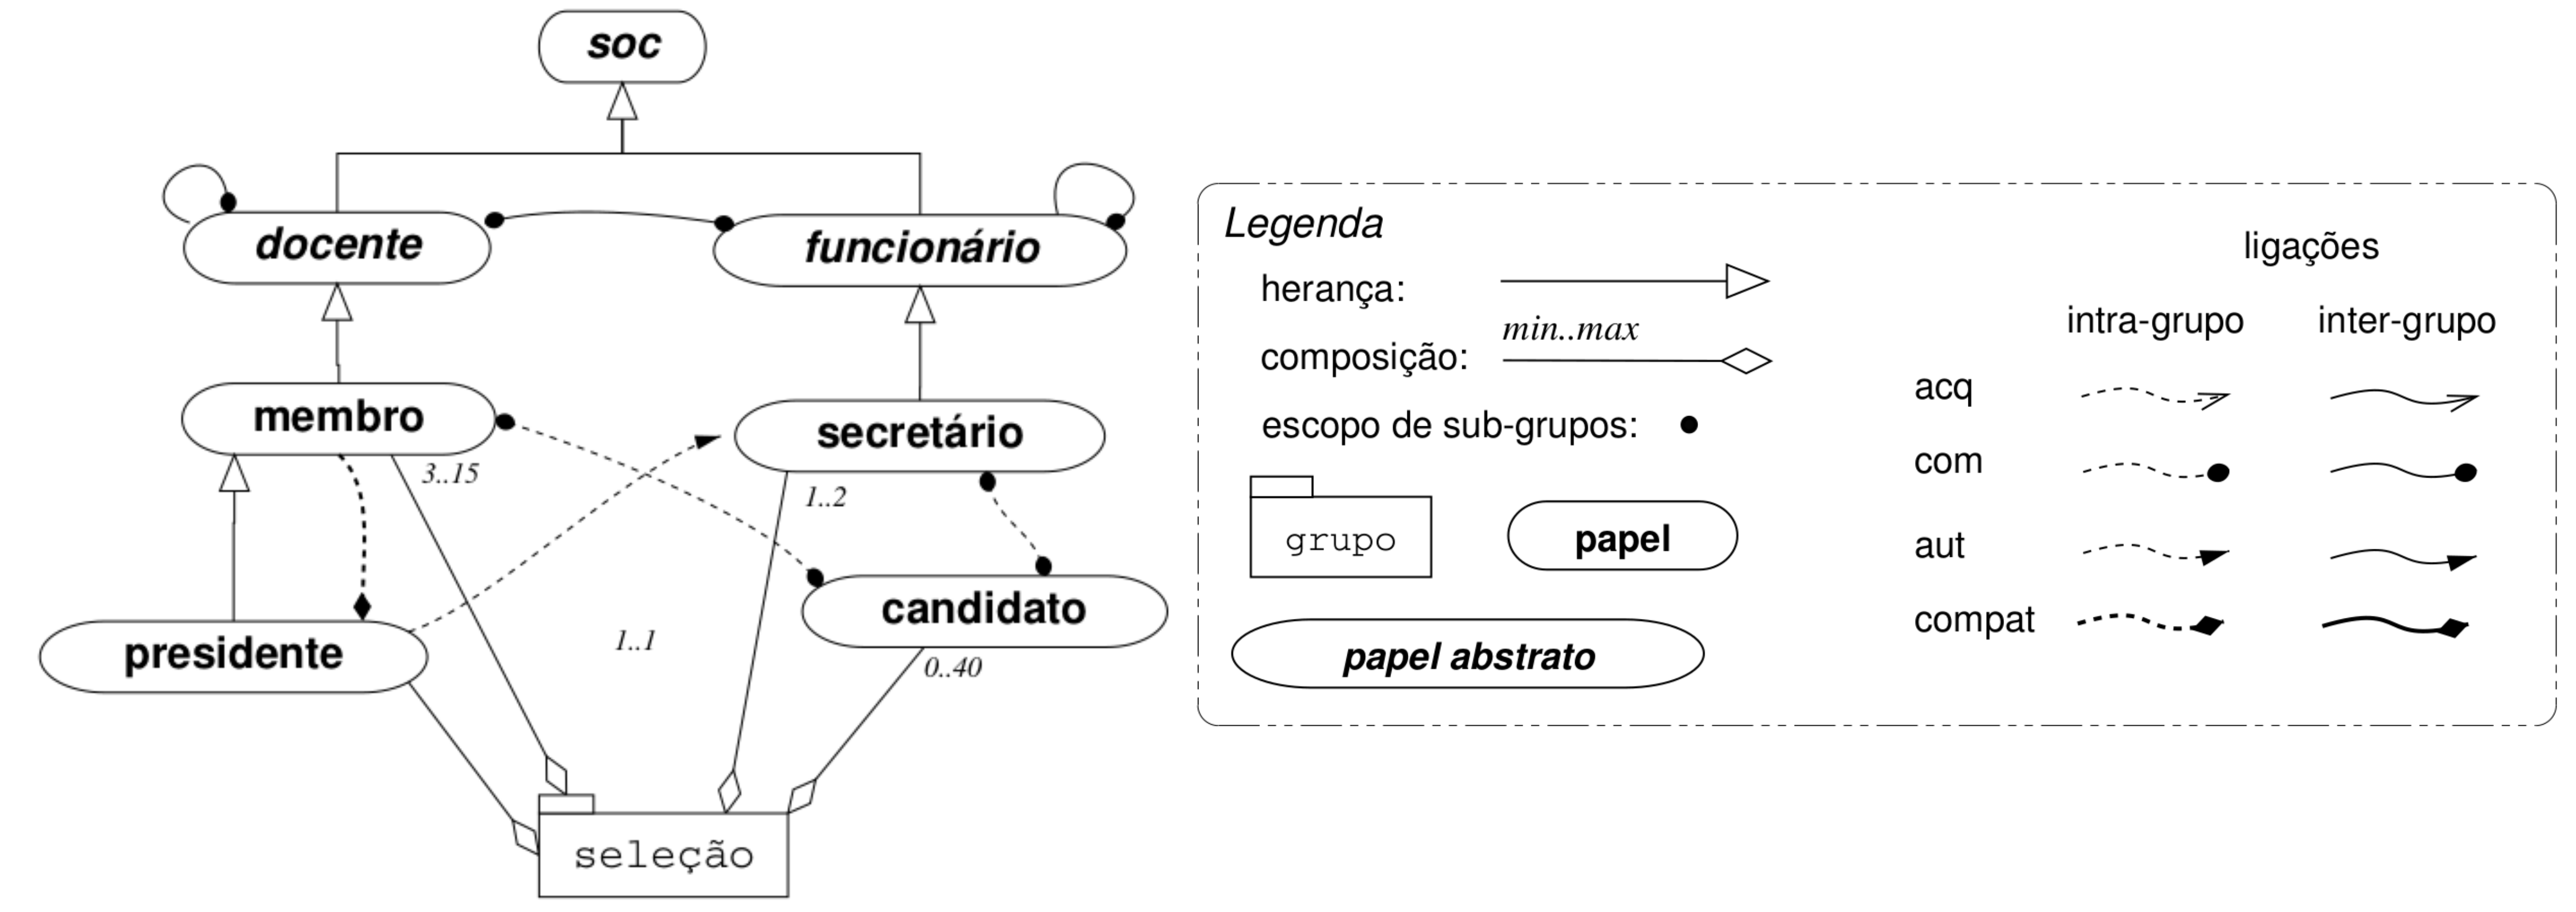
\includegraphics[scale=0.35]{imagens/modelo3.png}
\caption{Especificação Estrutural \cite{hubner2003modelo}.}
\label{fig:ee_exemplo}
\end{figure}

%acho que essa primeira frase está com algum problema, quando ela diz "uma relação entre preferência entre missões". Ou está mal escrita, ou eu não entendi.

\item {\it Especificação Funcional (EF)}: é constituída por um conjunto de esquemas sociais e de uma relação entre preferência entre missões. Nos esquemas sociais a meta global é um conceito fundamental. No nível individual um esquema social é constituído por missões. A missão é o conjunto de metas globais que podem ser passadas a um agente através de um de seus papéis. No nível coletivo um esquema social é uma árvore de decomposição de metas globais, a raiz é meta do esquema social e a decomposição de metas é feita através de planos. A Figura \ref{fig:es_exemplo} representa o esquema social para o exemplo. A leitura do esquema social deve ser feita da esquerda para a direita e de baixo para cima. O operador \textit{sequência} significa que a meta $g2$ só pode ser realizada quando a meta $g1$ for satisfeita. O operador \textit{escolha} significa que a meta $g7$ será satisfeita se uma e somente uma das metas $g8$ ou $g9$ for satisfeita. O operador \textit{paralelismo}, significa que a meta $g4$ será satisfeita quando ambas as metas $g5$ e $g6$ forem alcançadas, mas as duas sub-metas podem ser buscadas em paralelo. 
\begin{figure}[ht]
\centering
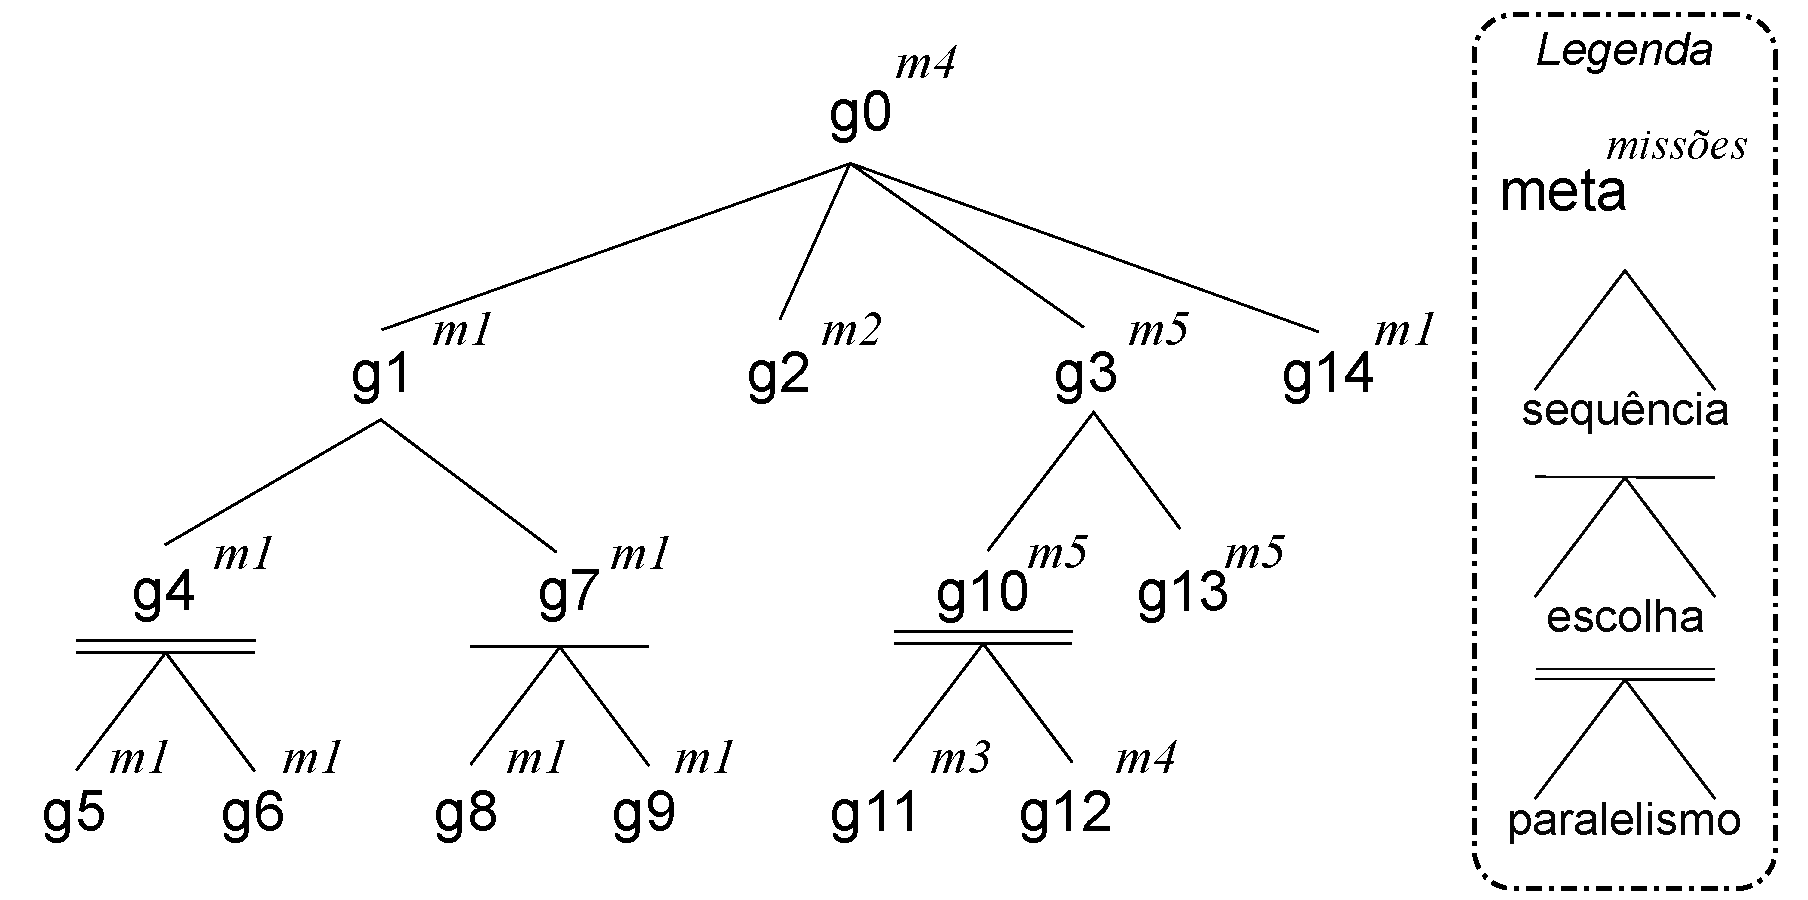
\includegraphics[scale=0.4]{imagens/ES2.pdf}
\caption{Esquema Social, adaptado de \cite{hubner2003modelo}.}
\label{fig:es_exemplo}
\end{figure}

Os diferentes papéis do exemplo possuem diferentes missões, um agente no papel de candidato, tem a missão $m1$. Para cumprir esta missão o candidato deve ter como objetivo as metas ($g1, g4, g5, g6, g7, g8, g9$ e $g14$), a descrição das metas está na Tabela \ref{tab:desc_metas}.

Portanto para cumprir a meta $g0$ primeiro o agente no papel candidato tem que ter toda a documentação necessária $g5$ e ter um orientador $g6$, com estas duas metas concluídas então a meta $g4$ é finalizada dando assim liberação para continuar, no caso para as metas $g8$ ou $g9$ já que o operador é de escolha.

Realizando a meta submissão eletrônica ($g8$) ou por correio ($g9$) a meta $g7$ está habilitada para ser concluída. Neste momento a meta $g1$ está liberada para ser satisfeita. A meta $g2$ faz parte da missão $m2$ que corresponde ao papel secretário, então um agente que assumir o papel de secretário da comissão deverá verificar se a documentação está correta.

As metas $g11$ e $g12$ podem ser realizadas em paralelo, e são responsabilidades do papel secretário $m3$ e do papel membro $m4$ respectivamente, assim que a metas estiverem concluídas, o presidente $m5$ assume a responsabilidade que $g10$ seja concluída, e terá que garantir que o projeto do candidato seja avaliado $g13$ e assegurar que seja aprovado pela comissão $g3$, ou reprovado caso ineficiente (um caso de falha na missão do candidato não descrito na especificação). E por fim o candidato tem a meta de garantir que o formulário de matrícula seja recebido pela comissão de seleção $g14$.

As relações das missões com os papéis podem ser observadas no item Especificação Deôntica logo abaixo.

\begin{table}[ht]
\footnotesize
\centering
\caption{Descrição das metas \cite{hubner2003modelo}.}
\label{tab:desc_metas}
\begin{tabular}{@{}llll@{}}
\toprule
meta   & \multicolumn{1}{l|}{descrição}                                       & meta & descrição                         \\ \midrule
g0     & \multicolumn{1}{l|}{candidato é aceito no programa de pós-graduação} & g7   & a inscrição está submetida        \\
g1(Dt) & \multicolumn{1}{l|}{a documentação é recebida no prazo}              & g8   & submissão eletrônica              \\
g2     & \multicolumn{1}{l|}{a documentação está correta}                     & g9   & submissão por correio             \\
g3     & \multicolumn{1}{l|}{candidato é aprovado pela comissão}              & g10  & metas g11 e g12 são cumpridas          \\
g4     & \multicolumn{1}{l|}{metas g3 e g4 são cumpridas}                                                & g11  & uma reunião está marcada          \\
g5     & \multicolumn{1}{l|}{candidato tem toda a documentação necessária}    & g12  & um relator está indicado          \\
g6     & \multicolumn{1}{l|}{candidato tem um orientador}                     & g13  & o projeto do candidato é avaliado \\
g14    & formulário de matrícula preenchido é recebido                        &      &                                   \\ \bottomrule
\end{tabular}
\end{table}

\item {\it Especificação Deôntica (ED)}: é a especificação que relaciona a EE com a EF no nível individual, especificando quais as missões um papel tem permissão ou obrigação de realizar. A Tabela \ref{tab:escola-deontica} contém a ED da sociedade comissão de seleção.

\begin{table}[ht]
\centering
\caption{Especificação deôntica. \cite{hubner2003modelo}}
\label{tab:escola-deontica}
\begin{tabular}{@{}lll@{}}
\toprule
papel       & relação deôntica  & missão                        \\ \midrule
candidato   & permissão         & \textit{m1}                          \\
secretário  & permissão         & \textit{m2}                          \\
secretário  & permissão         & \textit{m3}                          \\
membro      & permissão         & \textit{m4}                          \\
presidente  & permissão         & \textit{m5}                          \\
\bottomrule
\end{tabular}
\end{table}

\end{itemize}

\section{Teste de Software}

O teste faz parte dos métodos de verificação e validação de software onde a verificação investiga se o software atende aos seus requisitos funcionais e não funcionais enquanto a validação é um processo mais amplo no qual o objetivo é garantir que o software atenda às expectativas do cliente, sendo essencial já que nem sempre as especificações dos requisitos refletem os desejos ou necessidades reais dos clientes e usuários do sistema \cite{sommerville2010}. O termo garantir refere-se ao processo que visa obter confiança de que um sistema se comportará adequadamente \cite{winikoff2010assurance}. 

Segundo \citet{sommerville2010} o processo de verificação e validação possui outras atividades além dos testes, entre elas as inspeções e revisões de software. Estas atividades analisam e verificam os requisitos do sistema, os modelos de projeto, o código-fonte do programa e os testes propostos para o sistema como descrito na Figura \ref{fig:ver&val}. 

\begin{figure}[ht]
\centering
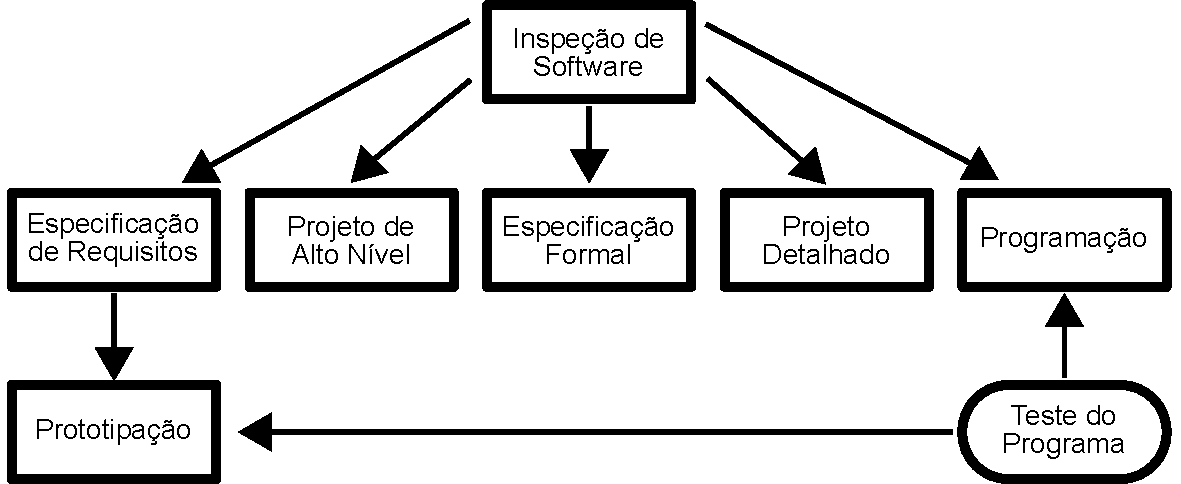
\includegraphics[scale=0.7]{imagens/validacao_verificacao.pdf}
\caption{Processo de verificação e validação. Adaptada de \cite{sommerville2010}.}
\label{fig:ver&val}
\end{figure}

As inspeções podem ser mais eficientes nas descobertas de defeitos do que os testes de software e possuem vantagens, como ser utilizada em  versões incompletas do sistema e podem ser inspecionadas sem necessidade de desenvolvimento de um teste específico. Os defeitos encontrados em uma inspeção podem considerar outros atributos de qualidade para um programa. A inspeção é um processo estático e não  tem  preocupação com as interações entre erros. Em testes dinâmicos muitas vezes um erro pode encerrar o sistema ou o próprio teste, e consequentemente uma única sessão de inspeção pode descobrir muitos erros em um sistema. 

No entanto, as inspeções não podem substituir os testes de software, pois não são eficazes para descobrir defeitos que surgem devido a interações inesperadas entre diferentes partes de um programa, problemas de temporização ou problemas com o desempenho do sistema. Além disso, pode ser difícil e dispendioso montar uma equipe de inspeção \cite{sommerville2010}. 

Teste de software é um processo, ou uma série de processos, elaborados para garantir que o código do computador realize o que foi projetado para fazer. O software deve ser previsível e consistente, sem oferecer surpresas aos usuários \cite{myers2011art}. Já para \cite{bourque2014guide} o teste é uma verificação dinâmica onde, em um conjunto de casos de testes finitos adequadamente selecionados dentro de um domínio de execução infinito, é analisado se o programa apresenta o comportamento esperado. Dentro deste conceito dinâmico significa que o teste requer sempre a execução do programa com entradas selecionadas.

O teste tem a função de medir a qualidade do software por pelo menos três termos: do número de defeitos encontrados, pelo rigor dos testes executados e pela cobertura do sistema pelos testes. Um teste deficiente pode revelar defeitos e passar falsa sensação de segurança. Um teste bem planejado irá revelar, em primeiro momento, defeitos se estiverem presentes e, se o teste passar, aumentará a confiança no software e será possível afirmar que o nível geral de risco de usar o sistema foi reduzido. Quando o teste encontra defeitos, a qualidade do sistema de software aumenta quando esses defeitos são corrigidos, desde que as correções sejam realizadas corretamente \cite{graham2008foundations}.


Antes de prosseguir alguns termos precisam ter suas definições apresentadas para evitar confusão. Conforme \cite{jorgensen2016software} as terminologias apresentadas nesta dissertação estão de acordo com \textit{International Software Testing Qualification Board} (ISTQB) e estas são compatíveis com os padrões do \textit{Institute of Electronics and Electrical Engineers} (IEEE) \textit{Computer Society} (IEEE, 1983).

\begin{itemize}
\item Erro (do inglês \textit{error}) - As pessoas cometem erros. Este erros podem ser cometidos durante a codificação por exemplo. Outros sinônimos em português podem ser engano ou equívoco.
\item Defeito (do inglês \textit{fault}) -  É o resultado de um erro. É mais preciso dizer que um defeito é a representação de um erro, onde a representação é o modo de expressão, sendo uma das formas de expressão um erro no código fonte, gerando uma anomalia (\textit{bug}) no funcionamento no sistema.
\item Falha (do inglês \textit{failure}) - É o resultado da execução de um defeito no código. As falhas também podem ser causadas por condições ambientais ou condições de \textit{hardware}.
\item Incidente - Ocorrência de evento que requer uma investigação. Um incidente é o sintoma associado a uma falha que alerta o usuário para a ocorrência de uma falha.
\item Caso de teste - um caso de teste possui um identificador e está associado ao comportamento de um programa. Ele também possui um conjunto de entradas e saídas esperadas.
\end{itemize}

Na Figura \ref{fig:processo_teste} é apresento um modelo abstrato do processo de teste tradicional, onde os casos de testes são especificações de entradas ao teste e onde é esperado uma saída com os resultados,  relacionado com uma declaração do que está sendo testado. Os dados de testes são as entradas que foram planejadas para testar o sistema, os resultados dos testes são automaticamente comparados com os resultados previstos não tendo necessidade de uma pessoa para verificar anomalias nesta etapa \cite{sommerville2010}.

\begin{figure}[ht]
\centering
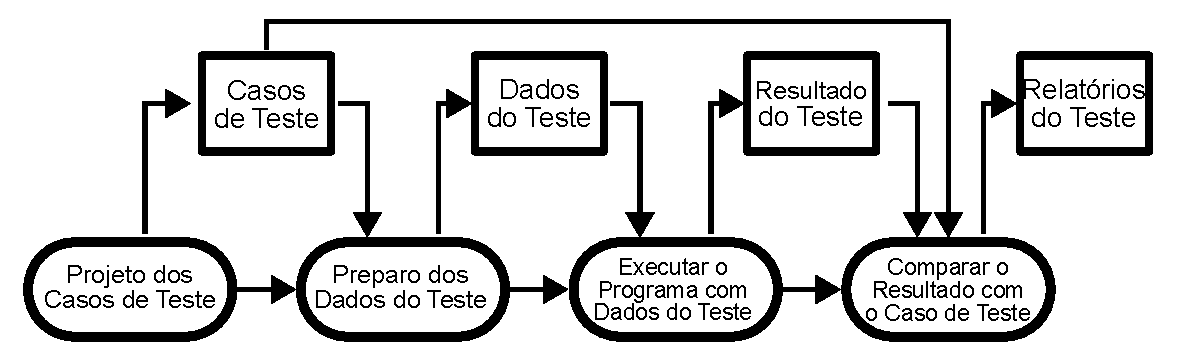
\includegraphics[scale=0.7]{imagens/processo_teste.pdf}
\caption{Modelo do processo de teste de software. Adaptada de \cite{sommerville2010}.}
\label{fig:processo_teste}
\end{figure}

Ainda sobre casos de testes, segundo \cite{myers2011art} é de grande importância um bom planejamento, já que é impossível realizar um teste completo. Um boa estratégia é tentar realizar o teste o mais completo possível dadas as restrições de tempo e custo. Levando isso em conta a questão-chave se torna: qual o subconjunto de casos de testes entre todos os casos de testes possíveis tem a maior probabilidade de detectar a maior parte das falhas? Em geral é impraticável, muitas vezes impossível, encontrar todos os erros em um programa. Este problema fundamental, por sua vez, terá implicações para a economia dos testes, os pressupostos que o testador terá que fazer sobre o programa e a maneira como os casos de teste são projetados.

Para encontrar um equilíbrio entre o menor número de casos de testes e uma ótima cobertura do programa são adotadas estratégias de teste de software. Uma estratégia para testes de software fornece um roteiro que descreve as etapas a serem realizadas como parte do teste, quando as etapas são planejadas, realizadas, e quanto esforço, tempo e recursos serão necessários. Portanto, qualquer estratégia de teste deve incorporar o planejamento do teste, a execução do teste e a coleta e avaliação de dados resultantes \cite{pressman2005software}.

Neste trabalho serão apresentadas duas abordagens que são utilizadas para identificar casos de testes, uma  baseada em especificação e tradicionalmente chamada de \textit{testes funcionais}, e outra baseada em código chamada de\textit{ testes estruturais} \cite{jorgensen2016software}. Os testes funcionais também são conhecidos por \textit{teste de caixa preta}, realizados na interface do software e com pouca consideração à estrutura lógica interna do software. Os testes estruturais, também conhecidos como \textit{teste de caixa branca}, são baseados em uma análise dos detalhes procedurais, os caminhos lógicos através do software e as colaborações entre componentes \cite{pressman2005software}.

\subsection{Teste de caixa preta}

O termo caixa preta é utilizado fazendo referência ao fato de que o projetista de testes não tem acesso ao código fonte do programa, sendo a parte interna do sistema desconhecida.  Assim o desenvolvimento do projeto de teste é realizado apenas tendo conhecimento da especificação do software. Para estes testes, a única informação utilizada é a especificação do software. Portanto os casos de testes são independentes de como o sistema é implementado, não gerando problemas se ocorrerem mudanças na implementação, e o desenvolvimento dos casos de teste pode ocorrer em paralelo com com a implementação \cite{jorgensen2016software}.

De acordo com \cite{pressman2005software}, com  nesta abordagem é possível obter um conjunto de condições de entradas que exercerão plenamente todos os requisitos funcionais de um programa. As principais fontes de erros encontrados são funções incorretas ou ausentes, erros de interfaces, erros em estruturas de dados ou acesso externo ao banco de dados, erros de comportamento ou desempenho e erros de inicialização e finalização do sistema.

Alguns dos pontos negativos dos testes baseados em especificação são que podem ocorrer redundâncias entre os casos de testes agravada pela possibilidade de partes do software que não foram testadas. E como os testes são baseados no comportamento especificado, é difícil de imaginar esses métodos identificando comportamentos que não são especificados \cite{jorgensen2016software}.

\subsection{Teste de caixa branca}

O nome caixa branca vem da exigência do conhecimento de como o software é implementado, enxergar o seu funcionamento interno. Para executar esta técnica, por exemplo, diferentes casos de testes podem ser derivados para um laço de repetição de um código, sendo independente da funcionalidade do software \cite{graham2008foundations}. Usando métodos de caixa branca é possível derivar casos de testes que garantem que todos os caminhos lógicos tenham sido executados pelo menos uma vez, como os lados verdadeiros e falso de uma decisão lógica, os laços de repetições e outras estruturas para garantir a sua validade \cite{pressman2005software}. Com os conceitos de teoria de grafo é possível descrever exatamente o que será testado. Esta técnica serve também para a definição e uso de métricas de cobertura de teste, indicando até que ponto o software foi testado oferecendo assim um melhor gerenciamento de teste \cite{jorgensen2016software}.

Entre os testes de caixa branca temos o teste de caminho ou \textit{path testing}, onde um programa é derivado (transformado) em um grafo direcionado em que os nós são fragmentos de declaração e as ligações, chamadas de arestas, representam o fluxo de controle. Para derivar um programa procedural em grafo de fluxo podemos usar a notação da Figura \ref{fig:4estrutura_basica} para cada uma das construções básicas da programação estruturada \cite{jorgensen2016software}.

\begin{figure}[ht]
\centering
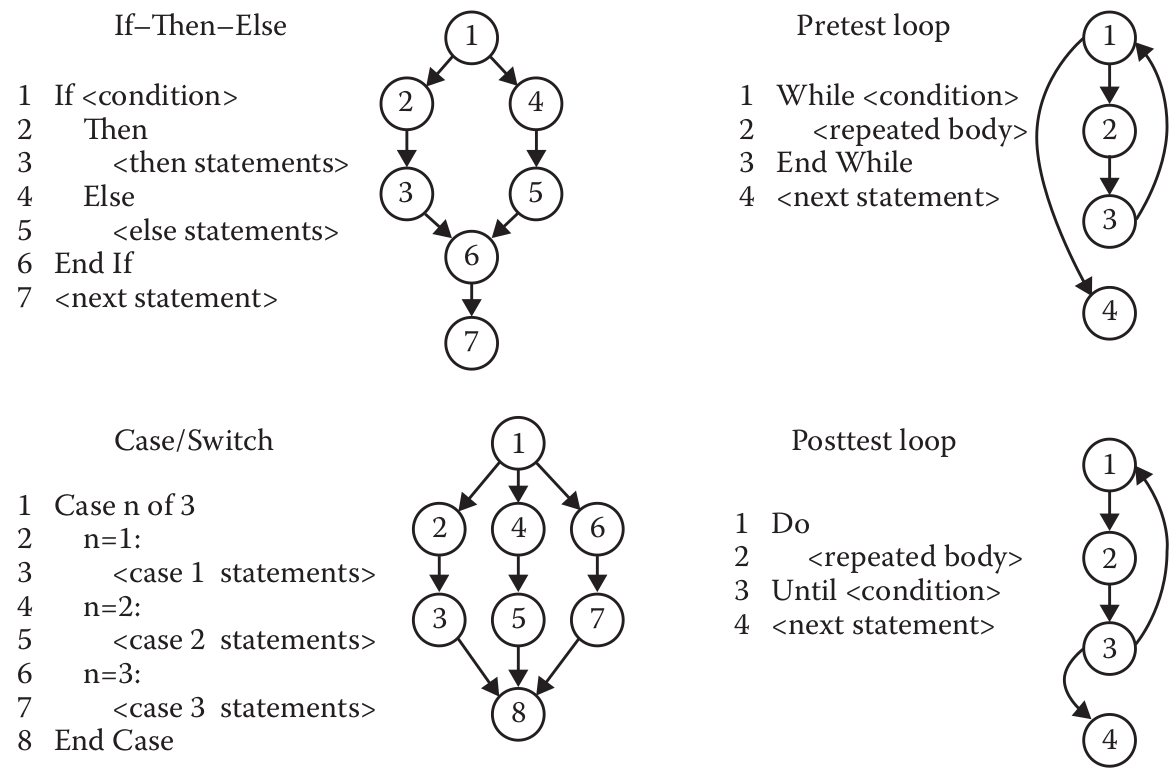
\includegraphics[scale=0.3]{imagens/const_basica_grafo.png}
\caption{Grafos para as quatro estruturas básicas da programação procedural \cite{jorgensen2016software}.}
\label{fig:4estrutura_basica}
\end{figure}

\cite{jorgensen2016software} define que um conjunto de casos de teste para um programa constituem a cobertura de nó. Quando executados no programa, cada nó no grafo é percorrido e constituem cobertura de aresta se, quando executado no programa, cada aresta do nó grafo for percorrida. \cite{winikoff2014testability} em seu trabalho apresenta um exemplo representado na Figura \ref{fig:exemplo_grafo}, onde existem 2 caminhos pelo programa ( 1, 2, 3, 5, 6) e (1, 2, 4, 5, 6). Um conjunto de testes para ser adequado deve ter pelo menos 2 casos de testes, um para exercitar cada caminho possível do programa.

\begin{figure}[ht]
\centering
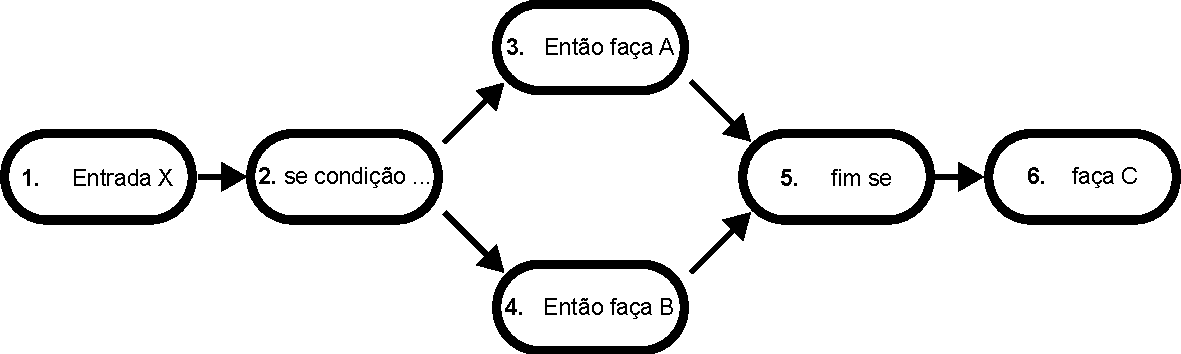
\includegraphics[scale=0.7]{imagens/exemplo_grafo.pdf}
\caption{Exemplo de grafo de fluxo de um programa. Adaptado de \cite{winikoff2014testability}}
\label{fig:exemplo_grafo}
\end{figure}


\subsection{Testes de sistemas no ciclo de desenvolvimento de software}

O projeto de testes para um software está diretamente relacionado ao modelo de ciclo escolhido para o desenvolvimento do sistema. Existem vários processos de desenvolvimento de software. Entre eles, modelo cascata, que possui as fases de análise e definição dos requisitos, projeto do sistema, implementação, integração e testes e por último entrega, operação e manutenção do sistema. Este modelo é bastante rígido e em princípio uma nova fase só começa quando a anterior termina \cite{sommerville2010}.

Existem outros modelos como o modelo iterativos, e modelos baseados em metodologias ágeis. Estes modelos especificam as várias etapas do processo e a ordem em que são realizados. A escolha  depende dos objetivos e metas do sistema a serem desenvolvidos, mas sempre levando em conta que a qualidade e confiabilidade são os principais fatores \cite{graham2008foundations}.

Os níveis de teste de software do \textit{V-Model} espelham o modelo cascata do ciclo de vida de desenvolvimento de software. Apesar deste modelo apresentar desvantagens como ter um ciclo de \textit{feedback} muito longo entre a especificação de requisitos e o teste do software e não prever suporte ao desenvolvimento paralelo no nível de unidade, ele é útil para identificar níveis distintos e esclarecer objetivos e responsabilidades para cada nível de teste. Uma variação do modelo cascata é apresentada na Figura \ref{fig:v-model} apresentando os níveis de testes relacionados a cada etapa do desenvolvimento \cite{jorgensen2016software}. 

\begin{figure}[ht]
\centering
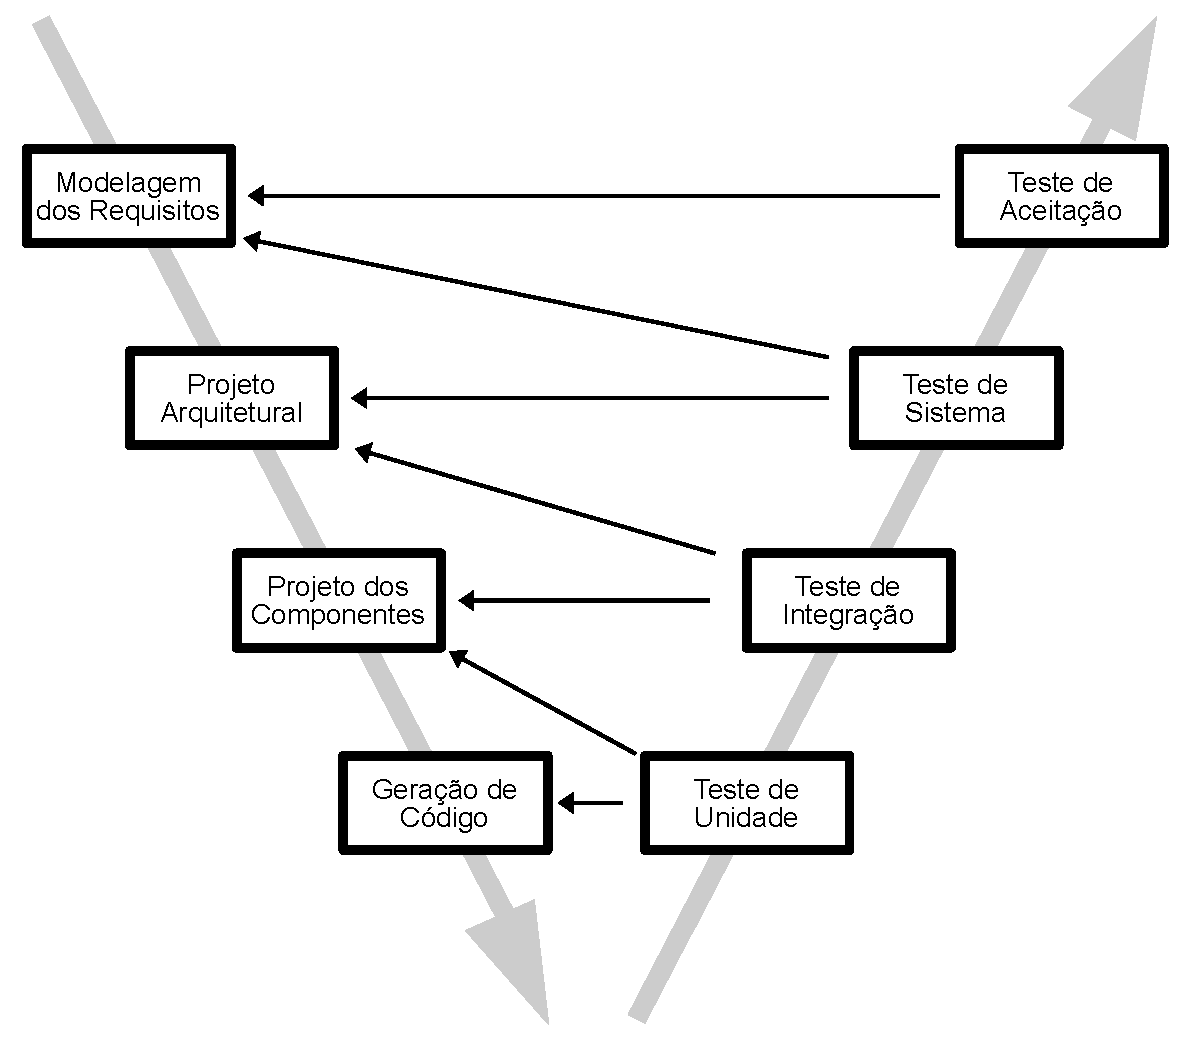
\includegraphics[scale=0.6]{imagens/v-model.pdf}
\caption{V-Model, adaptado de \cite{pressman2005software}.}
\label{fig:v-model}
\end{figure}

A grande contribuição do \textit{V-Model} foi a orientação de que o teste precisa começar o mais cedo possível no desenvolvimento do projeto. As atividades de testes devem ser realizadas em paralelo com as atividades de desenvolvimento, e toda a equipe deve trabalhar junta para que se possa identificar defeitos em decisões de projeto que de outra forma, separadamente, dificilmente seriam percebidas e comunicadas. A identificação precoce de defeitos é, de longe, o melhor meio de reduzir o seu custo final \cite{ammann2016introduction}.

\cite{graham2008foundations,ammann2016introduction} descrevem os níveis dos testes utilizados e seus objetivos:

\begin{itemize}
\item Teste de Aceitação: são projetados para determinar se o software atende aos requisitos e regras de negócio. Os testes são realizados com dados fornecidos pelo cliente do sistema e não com dados de teste simulados, e podem revelar erros e omissões na definição de requisitos do sistema, problemas de requisitos onde as instalações do sistema não atendem às necessidades do usuário ou desempenho do sistema inaceitável. Este nível de teste deve envolver o usuário ou alguém com conhecimento do domínio do sistema. 
\item Teste de Sistema: se preocupa com o comportamento do sistema e se ele está em conformidade com os requisitos definidos no projeto. Nesta etapa assume-se que as blocos de software estão funcionando de acordo, pois encontrar uma falha de nível inferior pode ter um grande custo para uma correção. Os testes geralmente são realizados por uma equipe específica para esta tarefa e não pelos programadores.
\item Teste de Integração: projetado para avaliar se a interação entre as interfaces dos módulos funciona corretamente. É uma técnica sistemática para a construção da arquitetura de software ao mesmo tempo que se investiga erros associados à interface. Uma das abordagens é construir o programa incrementalmente e cuidadosamente incluindo e testando os módulos de todos os componentes, assim erros são mais fáceis de isolar e corrigir. Geralmente é responsabilidade da equipe de desenvolvimento.
\item Teste de Unidade: avalia as unidades produzidas na fase de implementação. É o nível de teste que verifica as menores unidades do software como por exemplo classes, objetos e funções. Os erros encontrados pelos testes são limitados ao escopo estabelecido para o teste unitário,  concentrando-se na lógica do processamento interno.  É comum os testes unitários serem empacotados juntamente com o código fonte e serem utilizados para testes automáticos em outros momentos.
\end{itemize}


\section{Teste de Software em SMA} \label{sec:testesma}

Os agentes e sistemas multiagentes possuem muitas peculiaridades que tornam o processo de teste mais complexo e que devem abordar algumas questões que não eram preocupação no desenvolvimento de software orientado a objetos. Algumas dessas dificuldades foram citadas em \cite{rouff2002test,houhamdi2011multi,nguyen2009thesis} e são apresentadas a seguir, listando as propriedades específicas de agente ou SMA e o que ela gera de dificuldade em relação aos testes:

\begin{itemize}
\item Distribuído/assíncrono: os agentes podem operar de forma simultânea e assíncrona, ou seja, um agente pode ter que aguardar que outros agentes cumpram seus objetivos, e que o contexto permita a execução de seus planos. Um agente pode funcionar corretamente isolado, mas incorretamente quando colocado em uma comunidade de agentes ou vice-versa.
\item Autônomos: as mesmas entradas de testes podem resultar em comportamentos diferentes em diferentes execuções, uma vez que os agentes podem modificar sua base de conhecimento entre duas execuções ou podem aprender com entradas anteriores.
\item Envio de mensagens: os agentes se comunicam através de envio de mensagens. As técnicas de teste tradicionais, envolvendo chamadas de método, não podem ser aplicadas diretamente.
\item Fatores ambientais e normativos: o ambiente e convenções (normas, regras e leis) são fatores importantes que definem ou influenciam os comportamentos dos agentes. Alterações do contexto podem alterar os resultados do teste, e eventualmente, um contexto dá meios para que os agentes se comuniquem ou pode ser utilizado como uma entrada de teste.
\item Agentes “selados”: os agentes podem fornecer primitivas observáveis ou não ao mundo exterior, resultando em acesso limitado ao estado e ao conhecimento dos agentes internos. Um exemplo poderia ser um SMA aberto que permite que agentes de terceiros acessem os recursos do SMA, semelhante ao funcionamento de APIs. Nestes casos, é difícil garantir que estes agentes de terceiros com o conhecimento limitado sobre suas intenções tenham um comportamento apropriado.
\end{itemize}

Testar um único agente é diferente de testar uma comunidade de agentes. O teste de agentes pode ser feito de modo incremental durante o desenvolvimento testando funcionalidades à medida que elas são adicionadas. Alguns dos principais erros ao desenvolver agentes podem ser endereçar incorretamente uma mensagem para outro agente, enviar uma solicitação incorreta em uma mensagem ocorrendo que o agente receptor não reconheça a mensagem, analisar incorretamente mensagens recebidas, enviar uma mensagem ao agente errado, ou até mesmo não ter desenvolvido códigos do agente para que ele seja capaz de aceitar todas as mensagens \cite{rouff2002test}. Outros testes a serem realizados são verificar se a comunicação com o ambiente está correta e se a aprendizagem está adequada.

\begin{figure}[ht]
\centering
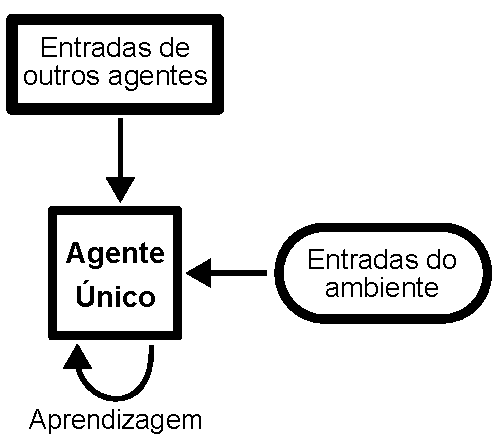
\includegraphics[scale=0.7]{imagens/single_agent.pdf}
\caption{Teste em um Agente, adaptado de \cite{rouff2002test}.}
\label{single}
\end{figure}

Testar uma comunidade de agentes torna os objetivos de testes mais amplos, tendo que verificar se os agentes da comunidade trabalham juntos como projetado, atestando a troca de comunicação entre eles, averiguando se essa troca de mensagem realmente está ocorrendo entre os agentes previstos  e  com o ambiente, mas agora com um agravante de ter um número muito maior de interações. \cite{rouff2002test} cita os erros mais observados em programadores desenvolvendo comunidades de agentes:

\begin{figure}[ht]
\centering
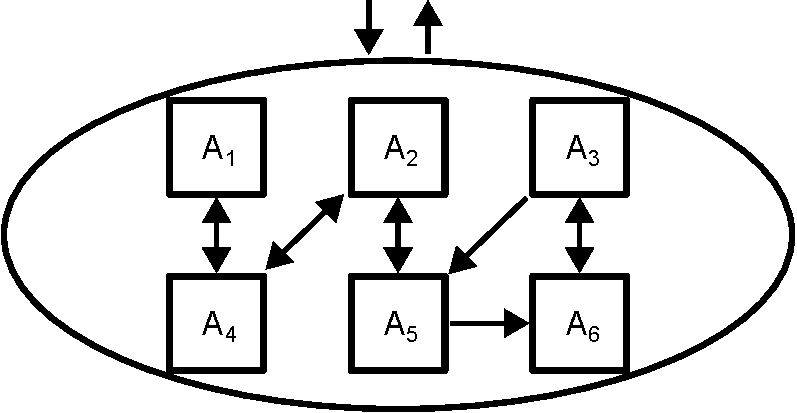
\includegraphics[scale=0.7]{imagens/community_agents.pdf}
\caption{Teste em comunidade de agentes, adaptado de \cite{rouff2002test}.}
\label{comunity}
\end{figure}

\begin{itemize}
\item Não documentar adequadamente as interações do agente, de modo que diferentes desenvolvedores implementam as interações de forma diferente.
\item Erro na mensagem, não comunicando o remetente, o conteúdo, entre outros, nas mensagens do agente.
\item Projetando impasses nas trocas de mensagens.
\item Não implementando mudanças nas mensagens para todos os agentes ao mesmo tempo (o que dificulta o teste da comunidade).
\end{itemize}

Para uma melhor organização, assim como os testes no ciclo de vida de desenvolvimento de software tradicional, os testes nos SMA também possuem vários níveis. O teste de unidade possui o mesmo nome nas duas abordagens, já o segundo nível é o teste de agente e não possui um relacionado. O teste de  grupo se relaciona com o teste de integração, o teste de sociedade está relacionado com o teste de sistema. E por último e com o mesmo nome tem o teste de aceitação \cite{houhamdi2011multi}. 

Os testes de unidade certificam-se que as menores unidades que compõem o agente estejam funcionando de acordo com o que foi planejado. Essas unidades incluem os blocos de código que implementam as metas, planos, base de conhecimento, mecanismos de raciocínio, especificações de regras entre outros. Já os testes de agentes testa a integração destas pequenas unidades  dentro do agente, verificando se os agentes são capazes de cumprir suas metas e se interagem corretamente com o ambiente. O teste de grupo avalia a interação entre agentes, protocolo de comunicação e semântica, integração com o ambiente, integração de agentes com recursos compartilhados, observa propriedades emergentes e comportamentos coletivos. Este teste certifica que um grupo de agentes e o ambiente funcionem corretamente juntos. O teste de sociedade avalia o SMA em execução no ambiente operacional de destino, testa as propriedades emergentes e macroscópicas esperadas do sistema. E o teste de aceitação testa o SMA no ambiente de execução do cliente e verifica se ele atende aos objetivos esperados das partes interessadas \cite{nguyen2009thesis}.

\section{Rede de Petri}

 Redes Petri (RP) é uma ferramenta gráfica e matemática para a descrição e análise de processos concorrentes, assíncronos e paralelos que surgem em sistemas distribuídos. Como ferramenta gráfica ela pode auxiliar na comunicação visual como um fluxograma e sendo uma ferramenta matemática, é possível estabelecer equações de estados, equações algébricas e outros modelos matemáticos que regem o comportamento dos sistemas \citep{murata1989petri}. 

Este modelo foi proposto por Carl Petri para modelar a comunicação entre autômatos, utilizados para representar sistemas a eventos discretos. Um sistema discreto é caracterizado pelas alterações de estados que ocorrem em instantes precisos. Os conceitos básicos para a modelagem de sistemas discretos são \cite{cardoso1997redes}:

\begin{itemize}
\item Eventos: são momentos de observação e de mudanças de estado do sistema.
\item Atividades: são as caixas-pretas utilizadas para abstrair a evolução do sistema entre dois eventos.
\item Processos: sequência de eventos e atividades.
\end{itemize}

A Figura \ref{fig:rede_petri} representa uma RP simples. O grafo da rede modela as propriedades estáticas de um sistema, assim como um fluxograma representa as propriedades estáticas de um programa de computador. O grafo contém dois tipos de nós: os círculos chamados de \textit{lugares} e as barras, chamadas de \textit{transições}. Os nós são conectados por arcos direcionados de \textit{lugares} para \textit{transições} e de \textit{transições} para \textit{lugares} \cite{peterson1977petri}. 

Além destes dois elementos, uma RP ainda possui propriedades dinâmicas que são resultantes da sua execução. O elemento que atribui esta propriedade dinâmica é a \textit{ficha} \cite{peterson1977petri}. As fichas são indicadas por um ponto em um lugar. A \textit{ficha} pode representar um recurso em uma posição, ou uma estrutura de dados que se manipula por exemplo \cite{cardoso1997redes}.

\begin{figure}[ht]
  \centering
  \subfigure[]{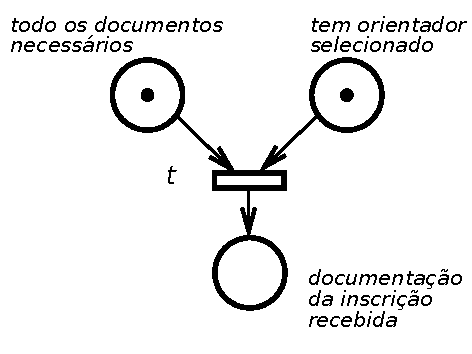
\includegraphics[width=0.45\textwidth]{imagens/2-petria.pdf}\label{fig:petria}}
  \subfigure[]{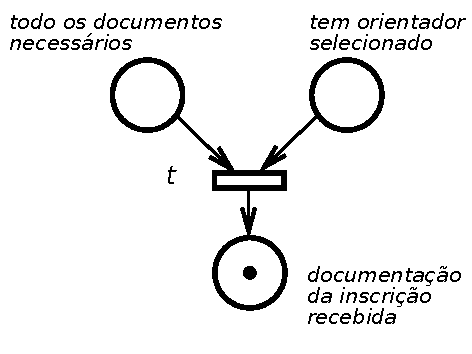
\includegraphics[width=0.45\textwidth]{imagens/2-petrib.pdf}\label{fig:petrib}}
  \caption{Rede de Petri}
  \label{fig:rede_petri}
\end{figure}

A dinâmica da RP atua da seguinte maneira.  As fichas são movidas pelo disparo das transições associadas da rede. Na Figura \ref{fig:petria} podemos observar que temos uma ficha no lugar \textit{todos os documentos necessários} e outra ficha em \textit{tem orientador selecionado}. A ocorrência do evento, associado à transição \textit{t} só pode ocorrer se houver ao menos uma ficha em cada um destes lugares. O disparo da transição \textit{t} retira uma das fichas vinculadas a cada um dos lugares de entrada e as posiciona no lugar de saída \textit{documentação da inscrição recebida} Figura \ref{fig:petrib}. A Figura \ref{fig:rede_petri} representa estados diferentes do mesmo sistema, uma evolução da rede, os arcos não apresentam nenhuma numeração indicando que o peso para disparar a transição é um, caso o peso para disparar a transição seja maior é necessário indicar o numeral no arco. 

As definições formais para Rede de Petri e Rede de Petri Marcada segundo \citet{cardoso1997redes} são:

\begin{definition}[Rede de Petri]
\label{drp}
Graficamente, uma Rede de Petri é uma n-tupla
\begin{equation}
R = \left \langle P, T, Pre, Post \right \rangle
\end{equation}
onde:
\begin{itemize}
\item $P$ é um conjunto finito de lugares de dimensão \textit{n};
\item $T$ é um conjunto finito de transições de dimensão \textit{m};
\item $Pre : P \times T \rightarrow \mathbb{N}$   é a aplicação de \textit{entrada} (lugares precedentes ou incidência anterior), com $\mathbb{N}$ sendo o conjunto dos números naturais;
\item $Post : P \times T \rightarrow \mathbb{N}$ é a aplicação de saída (lugares seguintes ou incidência posterior).
\end{itemize}
\end{definition}

\begin{definition}[Rede marcada]
  \label{drpmarcada}
  Uma rede marcada N é uma dupla

  \begin{equation}
      N = \left \langle R,M \right \rangle
  \end{equation}
  onde:
  \begin{itemize}
  \item $R$ é uma rede de Petri,;
  \item $M$ é a marcação inicial dada pela aplicação;
    \begin{equation}
        M : P \rightarrow \mathbb{N}
    \end{equation}
  \end{itemize}
\end{definition}

Para modelar sistemas complexos, onde por exemplo várias máquinas usam recursos diversos e podem trabalhar paralelamente fabricando peças diferentes,  é necessário dividir em várias RP ordinárias. Por não ter como diferenciar recursos e peças, já que as fichas são indiferenciáveis por obter apenas valores inteiros, as RP podem modelar o comportamento geral sem identidade de cada processo, faltando informação, ou modelar cada um dos processos individualmente e então modelar a interação entre eles, podendo ser muito trabalhoso ou tornando até mesmo ilegível \cite{cardoso1997redes, jensen2013coloured}.

Extensões para as RP ordinárias foram propostas para modelar sistemas complexos, cada uma com suas características, estes modelos são chamados de Redes de Petri de Alto Nível (RPAN). Neste trabalho o foco será nas Redes de Petri Coloridas (RPC), exposta na subseção seguinte.

\subsection{Redes de Petri Coloridas}

O benefício das RPC em relação as RP ordinárias é a possibilidade de utilização de marcas individualizadas (cores), que pode representar diferentes processos ou recursos de uma rede, permitindo a redução do tamanho de modelos \cite{maciel1996introduccao}. O uso dos conjuntos de cores nas RPC é semelhante aos tipos de dados das linguagens de programação (inteiro, real, caractere, lista) \cite{jensen2013coloured}.

Nas RPC cada lugar está associado a um conjunto de cores das fichas que podem pertencer a este lugar, cada transição se associa um conjunto de cores que podem dispara-lá e os arcos não possuem apenas o peso (valor inteiro), é necessário descrever quais cores de fichas serão retiradas do local inicial e quais cores de fichas serão colocadas nos lugares de saída.

Segundo \cite{maciel1996introduccao} as RPC são compostas por três partes distintas.

\begin{itemize}
\item Estrutura: é um grafo dirigido composto por vértices do tipo lugar, representado graficamente por círculos ou elipses e por vértices do tipo transição representado retângulos.
\item Declarações: são as especificações dos conjuntos de cores e declaração das variáveis.
\item Inscrições: os lugares possuem as inscrições nome, conjunto de cores e expressão de inicialização, estas são as fichas iniciais. As transições possuem as inscrições de nome e guarda que são restrições impostas pela transição. E os arcos possuem a inscrição de expressão, representando a ficha que será deslocada.
\end{itemize}

Para a modelagem das RPC será utilizada a ferramenta CPN Tools.

\subsection{CPN Tools}

CPN Tools é uma ferramenta para editar, simular e analisar redes de Petri Coloridas hierárquicas e temporais, ela possui uma interface flexível, técnicas de interação detalhadas e retornos gráfico que informam ao usuário sobre o status das verificações, simulações e sintaxes \cite{ratzer2003cpn}. Na Figura \ref{fig:cpn} é apresentada a interface gráfica da ferramenta com um exemplo de RPC.

\begin{figure}[ht]
\centering
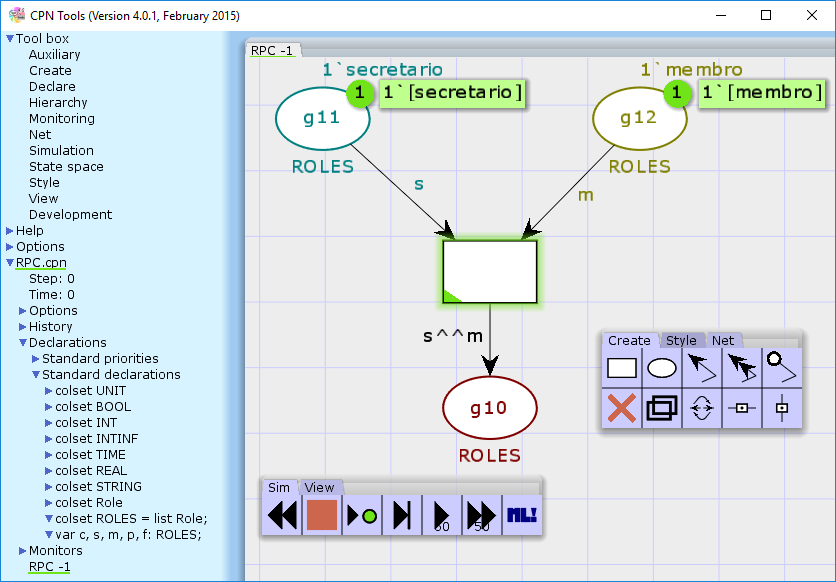
\includegraphics[scale=0.7]{imagens/2-cpn.png}
\caption{Interface do CPN Tools.}
\label{fig:cpn}
\end{figure}

A interface do programa possui um menu à esquerda. O item \textit{Tool Box} possui as caixas com as ferramentas para utilização do sistema, é possível colocar as caixas na área de trabalho clicando nelas e arrastando até o local desejado. Na Figura \ref{fig:cpn} é possível observar, à direita, duas caixas, uma delas com a aba \textit{Sim} selecionada mostrando as ferramentas de controle da simulação da RPC, e a aba \textit{View} em segundo plano, a outra caixa tem a aba \textit{Create} selecionada com as opções de criação da modelagem da RPC, e as abas \textit{Style} e \textit{Net} ambas em segundo plano, responsáveis  respectivamente por estilização da rede e por operações de gerenciamento de arquivo como salvar a rede atual.

O item RPC.cpn do menu é o nome do arquivo e dentro dele o item \textit{Declarations} se destaca, é no subitem \textit{Standard Declarations}, os conjuntos de cores \textit{UNIT}, \textit{INT}, \textit{STRING}, entre outras já são tipos declarados por padrão, e é possível definir outros tipo de declarações. Neste exemplo o código abaixo exibe por completo as declarações.

\begin{lstlisting}
colset Role = with candidato | secretario | membro | presidente;
colset ROLES = list Role;
var c, s, m, p: ROLES;
\end{lstlisting}

É definido um conjunto de cores \textit{Role} que possui quatro valores possíveis (candidato, secretario, membro, presidente), um conjunto de cores \textit{ROLES} que é uma lista de \textit{Role}, ou seja, aceita mais de uma cor por vez e a declaração das variáveis c, s, m, p to tipo \textit{ROLES}.

À direita é encontrada a área para modelagem da rede e o local onde as ferramentas de interação podem ser posicionadas. A rede modelada possui três \textit{lugares} cada um com a inscrição de seu nome $g11$, $g12$ e $g13$, todos  inscritos com o conjunto de cores \textit{ROLES} e os lugares $g11$ e $g12$ possuem expressão de inicialização, o primeiro uma ficha \textit{secretario} e $g12$ uma ficha \textit{membro}. Os lugares estão estilizados com cores diferentes mas esta configuração é apenas para melhor visualização da rede.

Os arcos possuem a inscrição de expressão que determina as fichas que irão sair dos lugares iniciais e que irão para o lugar final, a expressão $s^^m$ significa que a transição só vai ser ativada quando chegar na transição uma variável $s$ e e outra $m$ e ao sair da transição elas se tornarão uma lista. A transição $T1$ possui apenas a inscrição de nome, a borda e canto inferior esquerdo verde é um retorno que o CPN Tools dá de que a transição está ativada, ou seja, tem todos os requisitos para ser disparada.

Nativamente RP no CPN Tools não possui uma avaliação para contagem de caminhos, a solução para mensurar quantos caminhos tem uma RPC é avaliá-la como um grafo, construindo um grafo de marcações acessíveis. Os grafos possuem diversos algoritmos para contagem de caminhos, menor caminho, entre outros. 

As RP são grafos direcionados onde $G = (V, E)$ consiste em um conjunto $V$ de nós e um conjunto $E$ de arcos tal que cada arco $e \in E$ é associado a um par de nós não ordenados. Os caminho em grafos tem a seguinte definição de: considere $v_{o}$ e $v_{n}$ nós de um grafo. Um caminho de $v_{o}$ a $v_{n}$ de comprimento $n$ é uma sequência alternada de $n$+1 nós e $n$ arcos começando em $v_{o}$ e terminando em $v_{n}$ \cite{cardoso1997redes}. As RP
  

\subsection{Redes de Petri e SMA}

Diversos trabalhos utilizam RP no domínio de SMA. Em \cite{kohler2001modelling} RPC executáveis foram utilizadas para modelar a estrutura e o comportamento dos agentes. \citet{weyns2002colored} relataram como principais motivos da utilização de RPC como ferramenta de modelagem a visão conceitual clara sobre os agentes e o ambiente e o ótimo suporte a verificação e formalização. \cite{bai2004colored} apresentaram uma abordagem baseada em RPC para formar protocolos de interação flexíveis entre agentes. No trabalho \cite{de2004formal} é introduzido um modelo formal para verificar os planos em um SMA, baseadas na modelagem, simulação e verificação do modelo de RP Coloridas Hierárquicas (RPCH). \cite{poutakidis2009debugging} apresentam ferramentas para geração de casos de teste para de teste de unidade e outra para depuração e monitoramento de sistemas de agentes em execução. \citet{goncalves2010approach} expõe um modelo de RP desenvolvida para especificar o conhecimento em agentes e SMA, independentemente de estruturas e formalismos de representação do conhecimento. \cite{miller2011test} especifica, e mostra como medir, o grau de detalhes de um conjunto de casos de teste através de um agente de deputação que age como um oráculo, para avaliar a correção de um teste e utilizar a representação da RP do agente como suporte para medidas de cobertura de teste.





























